\subsection*{Двумерная решётка -- одна частица}
\addcontentsline{toc}{subsection}{Двумерная решётка -- одна частица}

\textbf{Задание:}\\
Реализовать модель процесса случайного блуждания. Рассчитать среднеквадратическое отклонение, размах в определённом интервале и математическое ожидание. Построить гистограмму по получаемым координатам. Визуализировать процесс перемещения точки.\\

\textbf{Решение:}\\
В качестве вероятности перемещения вверх, вниз, вправо или влево была задана вероятность 0.25. Начальная точка была взята (0;0), количество наблюдений -- 1000. В соответствии с процессом случайного блуждания был промоделирован процесс. (Рисунок \ref{fig:random_walk6})
\begin{figure}[h]
	\centering 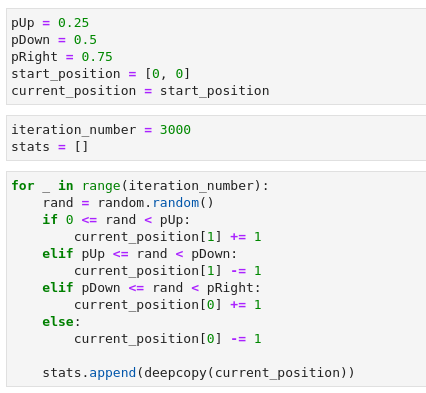
\includegraphics[scale=0.5]{random_walk6}
	\caption{Моделирования процесса случайного блуждания}
	\label{fig:random_walk6}
\end{figure}

Были рассчитаны основные показатели модели. (Рисунок \ref{fig:random_walk7})
\begin{figure}[h]
	\centering 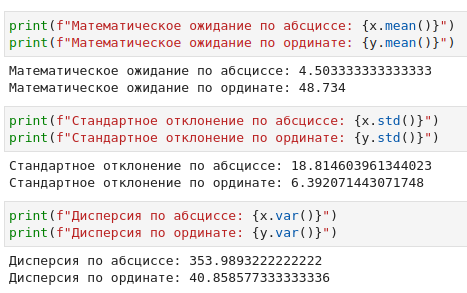
\includegraphics[scale=0.4]{random_walk7}
	\caption{Основные показатели модели}
	\label{fig:random_walk7}
\end{figure}

\newpage

Также был визуализирован процесс перемещения точки с течением времени. (Рисунок \ref{fig:random_walk8})
\begin{figure}[h]
	\centering 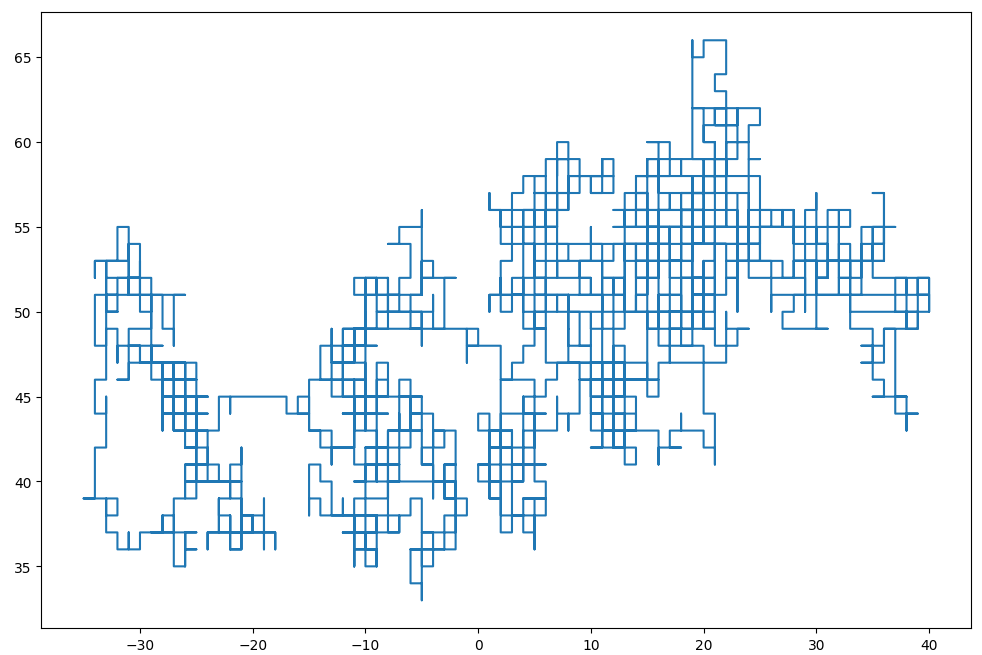
\includegraphics[scale=0.3]{random_walk8}
	\caption{Визуализация процесса перемещения точки с течением времени}
	\label{fig:random_walk8}
\end{figure}

Ещё была построена гистограмма, на которой показана частота встречаемости значений. (Рисунок \ref{fig:random_walk9})

\begin{figure}[h]
	\centering 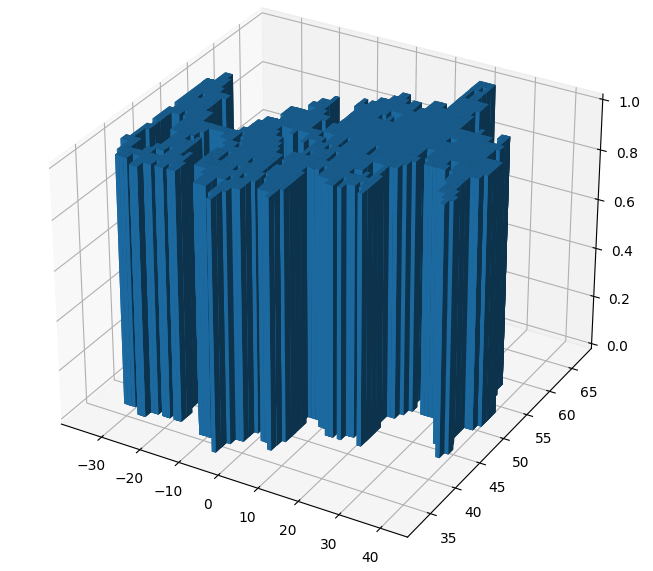
\includegraphics[scale=0.4]{random_walk9}
	\caption{Гистограмма по частоте встречаемости значений}
	\label{fig:random_walk9}
\end{figure}

Таким образом, был рассмотрен процесс случайных блужданий для двумерной решётки.